\subsection{ALMACD Development Diagram}
\label{subsec:almacd_diagram}
This section discusses the development and integration of the
Arnaud Legox Moving Average Convergence and Divergence (ALMACD)
indicator as a trading algorithm. The ALMACD indicator tells
traders when to buy and sell securities based on the convergence
and divergence of two ALMA (fast and slow). Specifically, when
the fast ALMA crosses above the slow ALMA, the indicator suggests
buying the stock. Conversely, when the fast ALMA crosses below
the slow ALMA, the indicator suggests selling the stock.
\hfill \\

The process of the development and integration of the ALMACD
is shown in Figure \ref{fig:almacd_diagram}.

% ALMACD Diagram
\begin{figure}[ht]
    \centering
    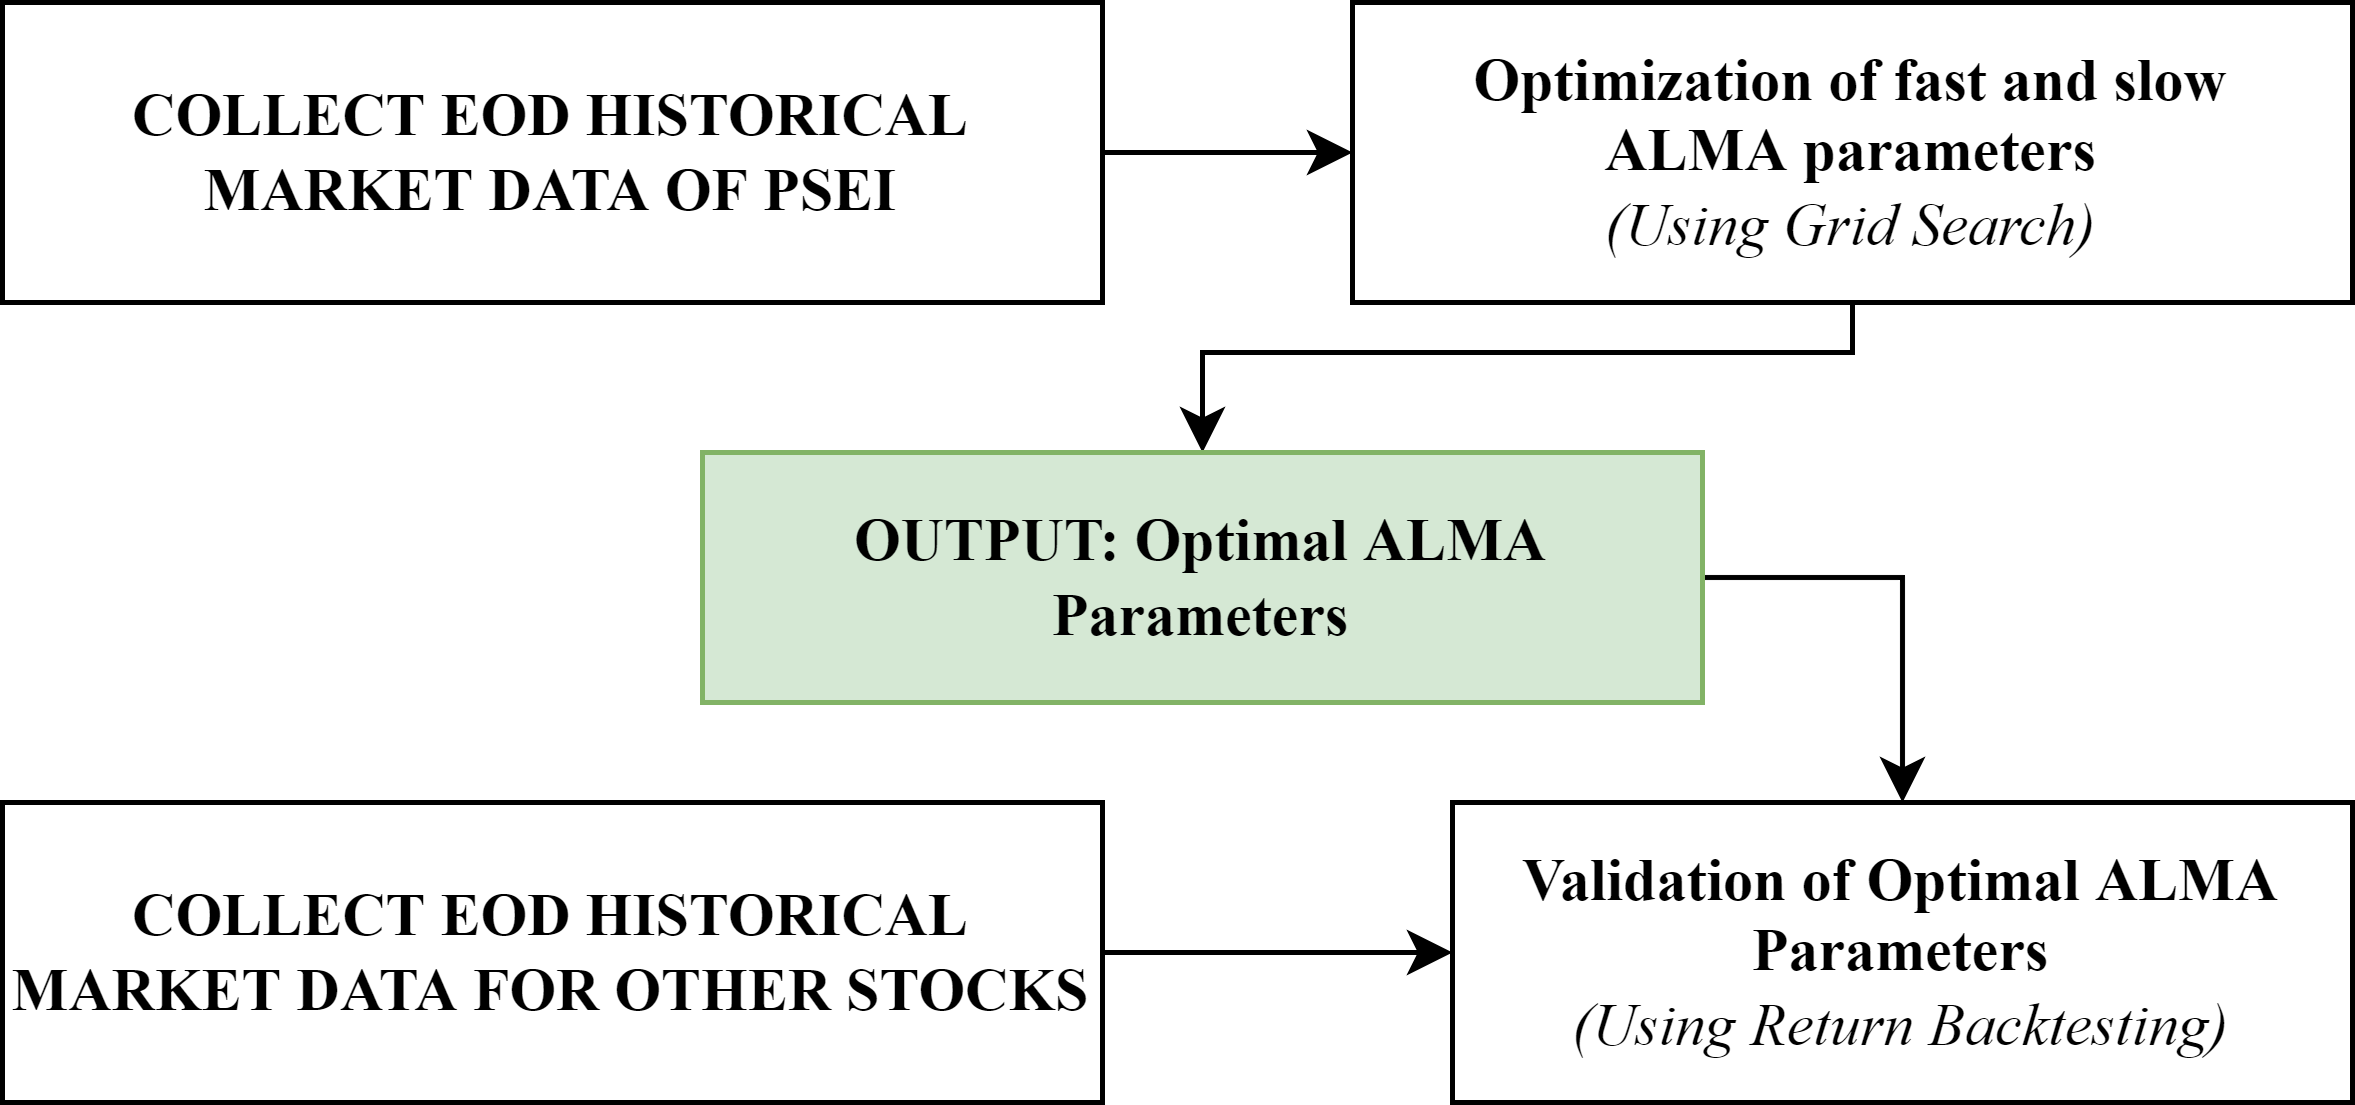
\includegraphics[width=0.80\textwidth]{./assets/Chapter_3/alamcd.png}
    \caption{ALMACD Development Methodology for alamSYS}
    \label{fig:almacd_diagram}
\end{figure}
\FloatBarrier

\subsubsection{Optimization of ALMA Parameters using Grid Search Approach}
\label{subsubsec:almacd_gridsearch}
The ALMACD indicator utilizes two ALMA indicators, one with a fast
period and one with a slow period. Where each of them have their own
set of optimal parameters, such as their window size, offset, and sigma.
In order to find this optimal parameters, a grid search approach was
used.
\hfill \\

Grid search is a machine learning technique used to fine-tune the
hyperparameters of a model. It is a brute force approach that tries
every combination of hyperparameters and evaluates the model performance
for each combination. The combination with the best performance is
then selected as the optimal hyperparameters \cite{Joseph2018}.
However in the case of the optimization of ALMACD, the grid search
approach was utilized to find the optimal parameters for the 
fast and slow alma, such that it yields a favorable performance
by computing the expected return of the trading algorithm. Whereas
the following parameters were used for the grid search approach:
\begin{itemize}
    \item For the fast ALMA:
    \subitem window size: a range from 1 to 10
    \subitem sigma: a range from 1 to 20
    \subitem offset: 0.85, 0.90, and 0.95
    \item For the slow ALMA:
    \subitem window size: a range from 10 to 20
    \subitem sigma: a range from 1 to 20
    \subitem offset: 0.85, 0.90, and 0.95
\end{itemize}

\subsubsection{Validation of ALMACD Parameters Using Return Backtesting Approach}
\label{subsubsec:almacd_validation}
Before integrating the optimal ALMACD parameters to the alamSYS, it was
first validated using the data from other stocks through backtesting, 
and calculating the potential returns. Once the
returns on the validation stocks were computed to be positive,
the ALMACD indicator was then integrated to the alamSYS.


\subsubsection{Integration of ALMACD to the alamSYS}
\label{subsubsec:almacd_integration}
The ALMACD indicator was integrated to the alamSYS as a trading
algorithm. It was implemented to run after the deep learning model
to better identify which stocks to buy and sell.